\documentclass[a4paper,12pt]{article}
\usepackage{amsmath, amsthm}
\usepackage{datetime}
\usepackage{framed}
\usepackage{enumitem}
\usepackage{fancyref}
\usepackage{wrapfig}
\usepackage{pifont}
\usepackage{appendix}
\usepackage{caption}
\usepackage{amsmath, amsthm, amssymb}
\usepackage{xcolor}

\usepackage{tikz}
\usetikzlibrary{fit,arrows,calc}
\usepackage{pgfplots}
\pgfplotsset{compat=1.8}

\usepackage{csquotes}
\renewcommand{\mkbegdispquote}[2]{\itshape}

\newdateformat{nianyueri}{ \THEYEAR 年 \THEMONTH 月 \THEDAY 日 }

\usepackage{data/circledsteps}
\usepackage[top=1in,bottom=1in,left=1in,right=1in]{geometry} % 用于设置页面布局
\usepackage{xeCJK} % 用于使用本地字体
\usepackage[super, square, sort&compress]{natbib} % 处理参考文献
\usepackage{titlesec, titletoc} % 设置章节标题及页眉页脚
%\usepackage{xCJKnumb} % 中英文数字转换
\usepackage{amssymb}
\usepackage{amsmath} % 在公式中用\text{文本}输入中文
\usepackage{diagbox}
\usepackage{multirow} % 表格中使用多行
\usepackage{booktabs} % 表格中使用\toprule等命令
\usepackage{rotating} % 使用sidewaystable环境旋转表格
\usepackage{tabularx}
\usepackage{graphicx} % 处理图片
\usepackage{footnote} % 增强的脚注功能,可添加表格脚注
\usepackage{threeparttable} % 添加真正的表格脚注,示例见README
\usepackage{hyperref} % 添加pdf书签

\usepackage{tikz}
\usetikzlibrary{shapes,arrows,shadows}

% 字体设置
\setmainfont{Times New Roman}
\setsansfont[Scale=MatchLowercase,Mapping=tex-text]{PT Sans}
\setmonofont[Scale=MatchLowercase]{PT Mono}
\setCJKmainfont[ItalicFont={Kaiti SC}, BoldFont={Heiti SC}]{Songti SC}
\setCJKsansfont{Heiti SC}
\setCJKmonofont{Songti SC}
% \setCJKmainfont[BoldFont={FZXiaoBiaoSong-B05S}]{Songti SC}
% \setCJKfamilyfont{kai}[BoldFont=Heiti SC]{Kaiti SC}
% \setCJKfamilyfont{song}[BoldFont=Heiti SC]{Songti SC}
% \setCJKfamilyfont{hei}[BoldFont=Heiti SC]{Heiti SC}
% \setCJKfamilyfont{fsong}[BoldFont=Heiti SC]{Songti SC}
% \newcommand{\kai}[1]{{\CJKfamily{kai}#1}}
% \newcommand{\hei}[1]{{\CJKfamily{hei}#1}}
% \setromanfont[Mapping=tex-text]{TeXGyrePagella}
% \setsansfont[Scale=MatchLowercase,Mapping=tex-text]{TeXGyrePagella}
% \setmonofont[Scale=MatchLowercase]{Courier New}
%%设置常用中文字号,方便调用
\newcommand{\erhao}{\fontsize{22pt}{\baselineskip}\selectfont}
\newcommand{\xiaoerhao}{\fontsize{18pt}{\baselineskip}\selectfont}
\newcommand{\sanhao}{\fontsize{16pt}{\baselineskip}\selectfont}
\newcommand{\xiaosanhao}{\fontsize{15pt}{\baselineskip}\selectfont}
\newcommand{\sihao}{\fontsize{14pt}{\baselineskip}\selectfont}
\newcommand{\xiaosihao}{\fontsize{12pt}{\baselineskip}\selectfont}
\newcommand{\wuhao}{\fontsize{10.5pt}{\baselineskip}\selectfont}
\newcommand{\xiaowuhao}{\fontsize{9pt}{\baselineskip}\selectfont}
\newcommand{\liuhao}{\fontsize{7.5pt}{\baselineskip}\selectfont}

% 章节标题显示方式及页眉页脚设置
% \item xCJKnumb是自己额外安装的包
% \item titleformat命令定义标题的形式
% \item titlespacing定义标题距左、上、下的距离
\titleformat{\section}{\raggedright\large\bfseries}{\thesection}{1em}{}
\titleformat{\subsection}{\raggedright\normalsize\bfseries}{\thesubsection}{1em}{}
\titlespacing{\section}{0pt}{*0}{*2}
\titlespacing{\subsection}{0pt}{*0}{*1}
% 由于默认的2em缩进不够,所以我手动调整了,但是在windows下似乎2.2就差不多了,或者是article中没有这个问题
\setlength{\parindent}{2.2em}

% 设置表格标题前后间距
\setlength{\abovecaptionskip}{0pt}
\setlength{\belowcaptionskip}{0pt}


\renewcommand{\refname}{\bfseries{参~考~文~献}} %将Reference改为参考文献(用于 article)
% \renewcommand{\bibname}{参~考~文~献} %将bibiography改为参考文献(用于 book)
\renewcommand{\baselinestretch}{1.38} %设置行间距
\renewcommand{\figurename}{\small\ttfamily 图}
\renewcommand{\tablename}{\small\ttfamily 表}


\usepackage{stmaryrd}
\usepackage{mathtools}
\usepackage{wasysym}

\newtheorem{definition}{定义}
\newtheorem{lemma}{引理}
\newtheorem{proposition}{命题}
\newtheorem{theorem}{定理}
\newtheorem{grammar}{文法}
\newtheorem{program}{程序}
\newtheorem{convention}{约定}
\renewcommand*{\proofname}{证明}

\xeCJKsetwidth{‘’“”}{1em}

\title{数字丛林里的远足\\
\large 从词向量到算术表达式的几何}
\date{2021 年 6 月}
\author{苑明理}

\begin{document}
\maketitle{}
\centerline{\rule{13cm}{0.4pt}}
\renewcommand{\contentsname}{\hfill\bfseries 目录\hfill}
\setcounter{tocdepth}{2}
\tableofcontents
\centerline{\rule{13cm}{0.4pt}}
\newpage

\section{引言}

几千年来,最基本的数学对象之一—算术表达式,一直都是以一种离散的方式存在。数通过四则运算连接在一起,构成了算术表达式,
除了一些代数变形可以连接不同的表达式,两个表达式 $A$ 和 $B$ 之间没有特别好的、几何的连接方式。
有没有算术表达式的几何化方式呢?本文我们将会给出一个思路的说明。

事情可以追溯到 2015 年底,当时我在上海短居。在考虑用词向量技术表达整数的时候,我发现可以构造一种有趣的、双曲平面上的离散结构。
当看到那些蜿蜒到无穷的折线和均匀的数值分布时,我意识到可能发现了一个有着丰富内涵的数学结构。其后的几年我一直在反复琢磨它。

2019 年 10 月底我去美国出差,11 月初在回国的飞机上,我偶然发现了这种构造方式可以推广到无穷小。
一两天后,我得到了双曲平面上无穷小生成结构的流方程。和中山大学的蒋文峰老师讨论后,他给到我很多好的建议,鼓励我一步步走下去。

2019 年底到 2020 年夏,我在努力把这个结果应用到一种重要的神经网络上—残差网络,可以得到一类特殊的网络架构来解决演化问题。
几个月的努力,逐步得到了一些有趣的神经网络架构,虽然在一些演化问题上它还没有达到工业界的最佳水平,但也有着良好的性能,
至少可以说明这种几何化的想法在实践中是可行的。这些应用角度的努力,也可以从理论角度给予解读,是在探索另外一种微积分的可能性。

2020 年底,在和英国的刘宇老师讨论后,他问了我几个特别好的问题,促使我重新思考,结果发现无穷小生成元的选择是自由的,
这样就导出了一个非常深刻的管型构造,这个管型构造能和多项式联系起来,是一种纤维结构。
但是这些几何构造还仅仅存在于设想中,它还欠缺一个严密的理论基础。

于是,在2021 年初,我从公司(彩云科技)争取了三个月的时间,在实习生张乐和张怀公的帮助下,我们一起找到了第一个严格的、
可以解算的实例(张乐的工作),也找到了一般情况下的表述方法(张怀公的工作)。

本文会沿着真实思路发展的线索,陈述这个算术表达式几何化的想法。

对这种几何化我们还有一种理解,算术表达式的计算过程包含了丰富的信息,远比一个简单的计算结果要重要得多。简单说,就是“过程比结果更重要”。
在此,我也想表达,如果我们的历程是一个数字丛林里的探险,那么这个探险是永远没有止境的,它的过程远比一个探险报告有趣的多。

\newpage

\section{词向量与数}

在计算语言学的研究中,从 1978 年 Salton 的 VSM 模型起 \cite{Almeida2019WordEA},人们为了方便计算,
常常把词汇表示成向量,并称这种表示为词嵌入。 2013 年 Mikolov 的论文 \cite{Mikolov2013EfficientEO} 发表后,
人们开始认识到,一类称为正则的嵌入方式是特别值得关注的,它们拥有一种组合性\cite{Mikolov2013DistributedRO}。
这里,我们把这种组合性归纳为:
\begin{enumerate}
\item 词和词之间的关系是有意义的
\item 同义的关系是平行的
\item 词和关系可以通过向量运算组合起来,形成一个格网
\end{enumerate}

\begin{figure}[ht]
\centering
\begin{tikzpicture}[x=0.5cm,y=0.5cm,z=0.3cm,>=stealth]
\draw[->] (xyz cs:x=-7.0) -- (xyz cs:x=7.0) node[above] {$x_0$};
\draw[->] (xyz cs:y=0) -- (xyz cs:y=7.0) node[right] {$x_n$};
\draw[->] (xyz cs:z=-7.0) -- (xyz cs:z=7.0) node[above] {$x_i$};

\node[fill,circle,inner sep=1.5pt,label={left:$king$}] (p) at (xyz cs:x=-3.0, y=3.0, z=-3.0) {};
\node[fill,circle,inner sep=1.5pt,label={right:$man$}] (q) at (xyz cs:x=2.0, y=-3.0, z=3.0) {};
\node[fill,circle,inner sep=1.5pt,label={left:$queen$}] (r) at (xyz cs:x=-3.0, y=3.0, z=3.0) {};
\node[fill,circle,inner sep=1.5pt,label={right:$woman$}] (s) at (xyz cs:x=2.0, y=-3.0, z=9.0) {};
\draw[dashed, blue] (p) -- (q);
\draw[dashed, blue] (r) -- (s);
\draw[dashed, red] (p) -- (r);
\draw[dashed, red] (q) -- (s);
\end{tikzpicture}
\caption{正则词嵌入的组合性}
\label{fig:compositionality}
\end{figure}

上图的示例可以简述为:男人、国王、女人、女王四个词形成一个平行四边形,其中有两对同义的关系
\begin{enumerate}
\item femalize:女性化的维度,从男人到女人、从国王到女王
\item royalize:皇权的维度,从男人到国王、女人到女王
\end{enumerate}

而几何上的平行四边形也可以通过$royalize$与$femalize$两个运算的可交换性来表达:
$$
    royalize(femalize(man)) = femalize(royalize(man))
$$

或者通过下面的交换子恒为零来表示
$$
    royalize(femalize(man)) - femalize(royalize(man)) = 0
$$

因为机器学习模型的统计特点,这里的组合性只是一种近似关系。机器学习界指出了组合性的存在,但并没有沿这个方向走太远。

整数和整数之间存在很多关系,但是如果我们把 $\cdot + 1$ 和 $\cdot \times 2$ 视为基本关系,我们能得到什么? 此时,我们发现:

$$
[(x + 1) \times 2] - (x \times 2 + 1) = 1
$$

这说明平行四边形永远无法存在。我们知道双曲空间是一种不存在平行四边形的空间,
简单尝试就可以把$\cdot + 1$关系、 $\cdot \times 2$关系和所有整数安排到双曲空间的一个网格上。

\begin{figure}[ht]
\centering
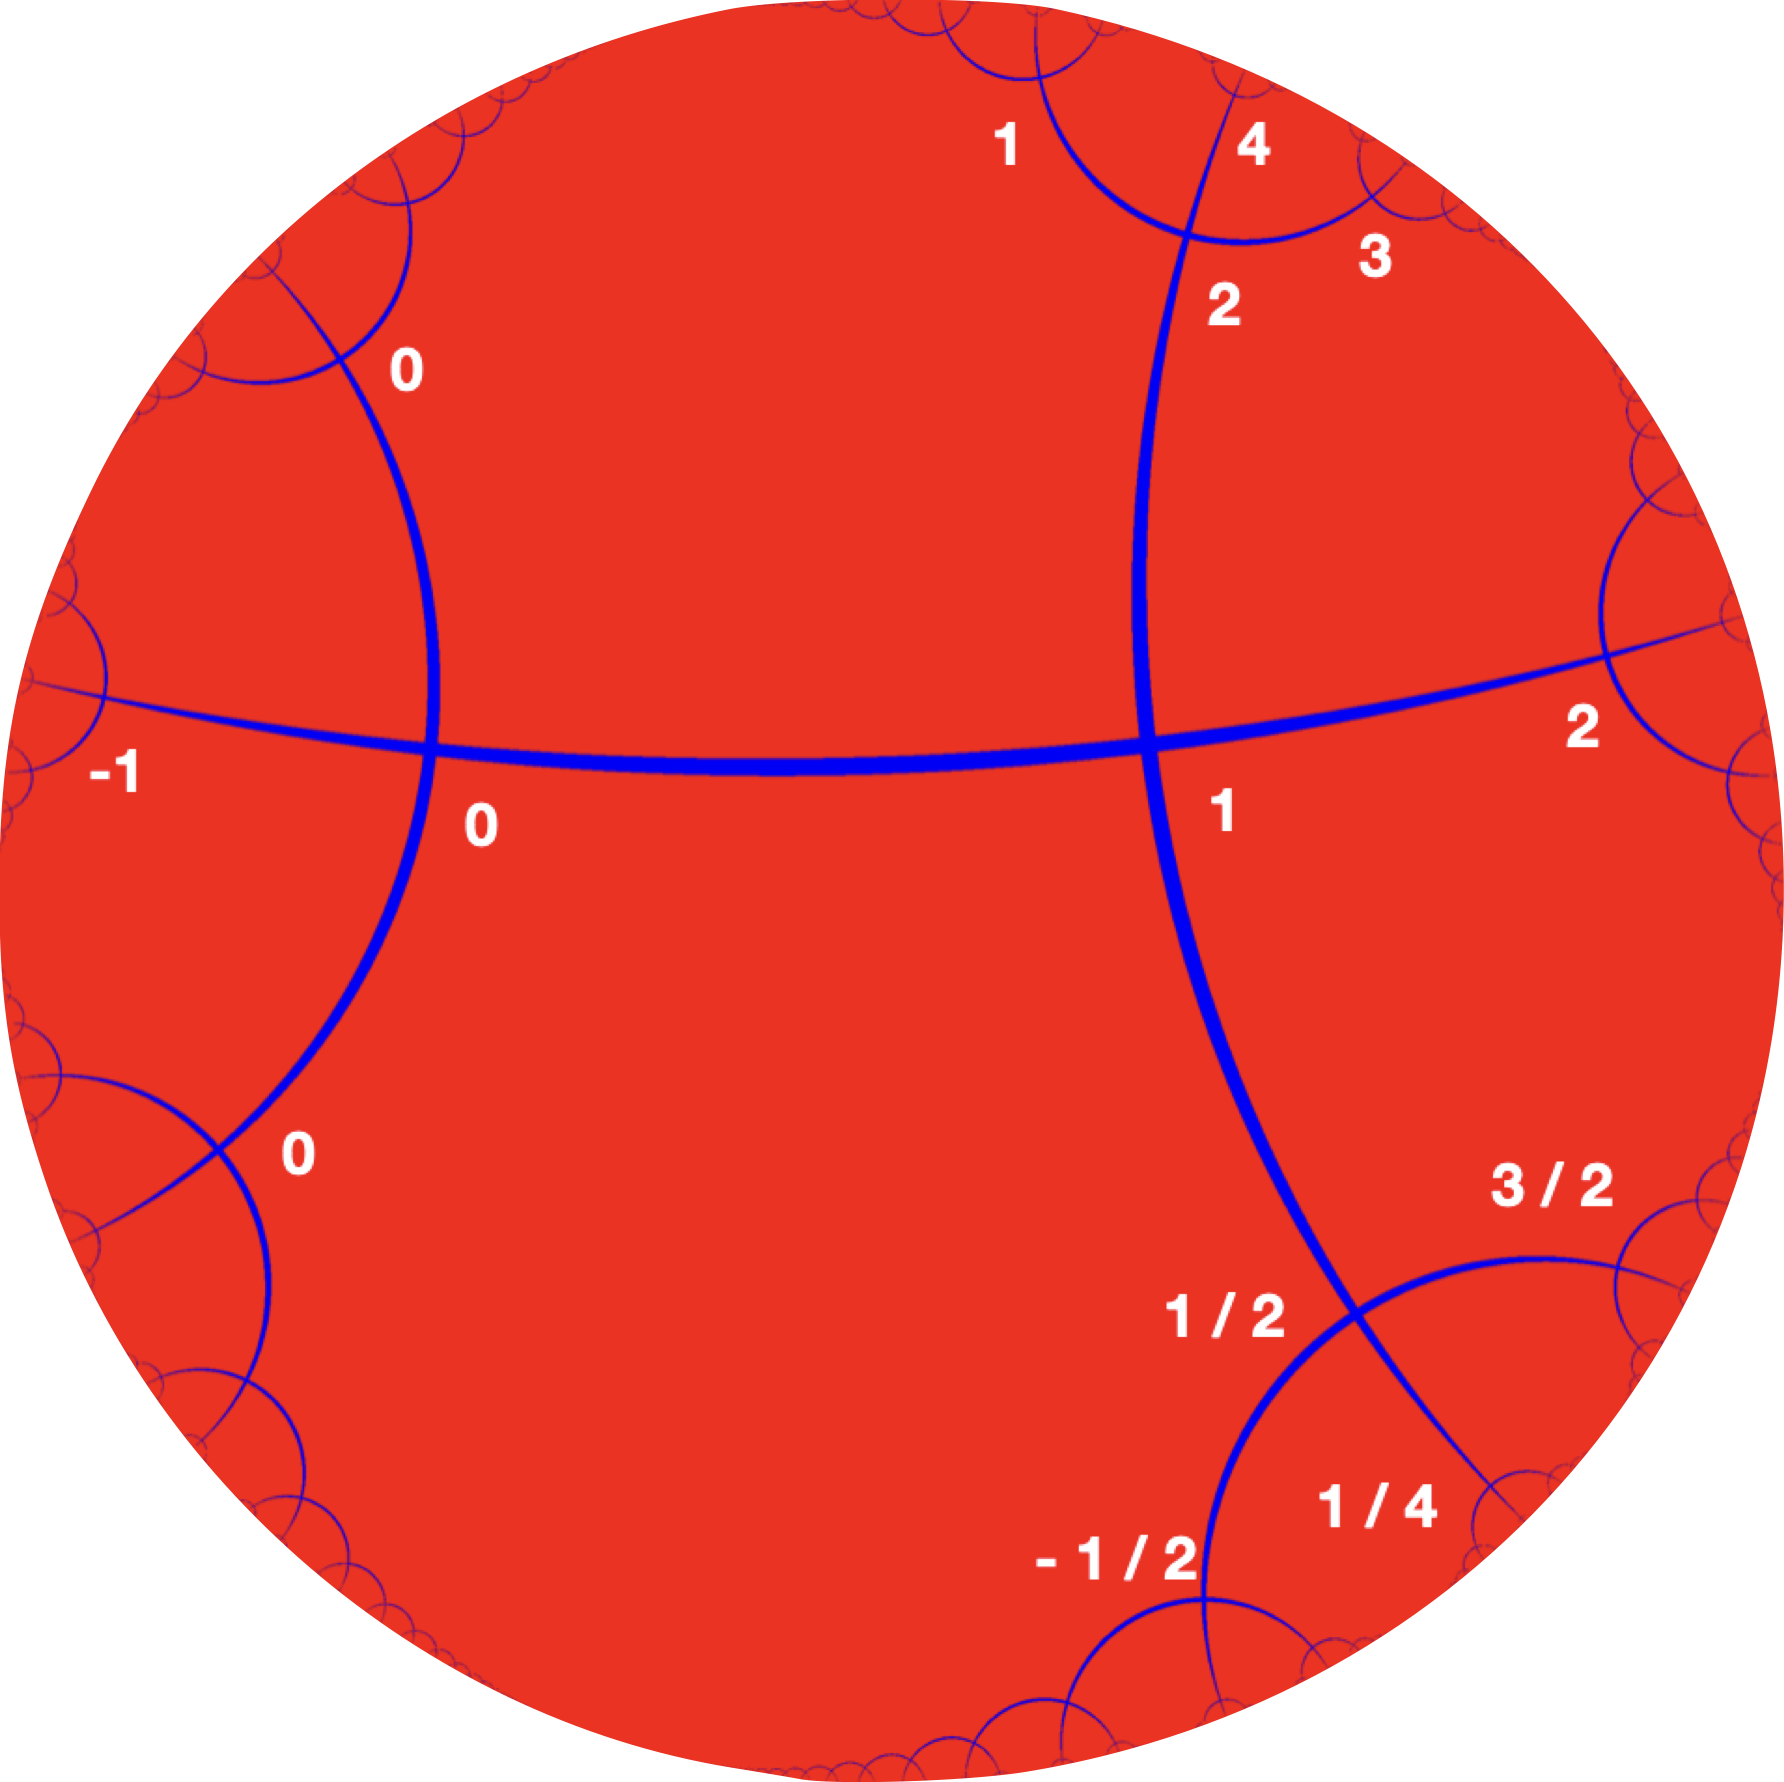
\includegraphics[width=4in]{images/assignment2.png}
\caption{$\cdot + 1$关系、 $\cdot \times 2$关系的赋值网格}
\end{figure}

这个网格的构造规则如下
\begin{enumerate}
    \item 网格呈现为四阶无限边形铺嵌
    \item 加乘轴相互垂直、交替出现
    \item 加轴、乘轴按右手系排布
\end{enumerate}

我们需要论证依照此程序,可以无矛盾的构造几何构形,直至无限边形的无穷远处。

\begin{theorem}
    加轴、乘轴赋予合适的增长方向,依照右手系(或左手系)可以排布满整个四阶无限边形铺嵌中的四阶凯莱树
\end{theorem}

\begin{proof}
对四阶无限边形铺嵌的节点、面染色
\begin{enumerate}
    \item 节点可以在黑、白两种选择中交错染色,且可以无矛盾地拓广至无穷远处;
    \item 面可以在红、蓝两种选择中交错染色,且可以无矛盾地拓广至无穷远处;
\end{enumerate}

\begin{figure}[ht]
\centering
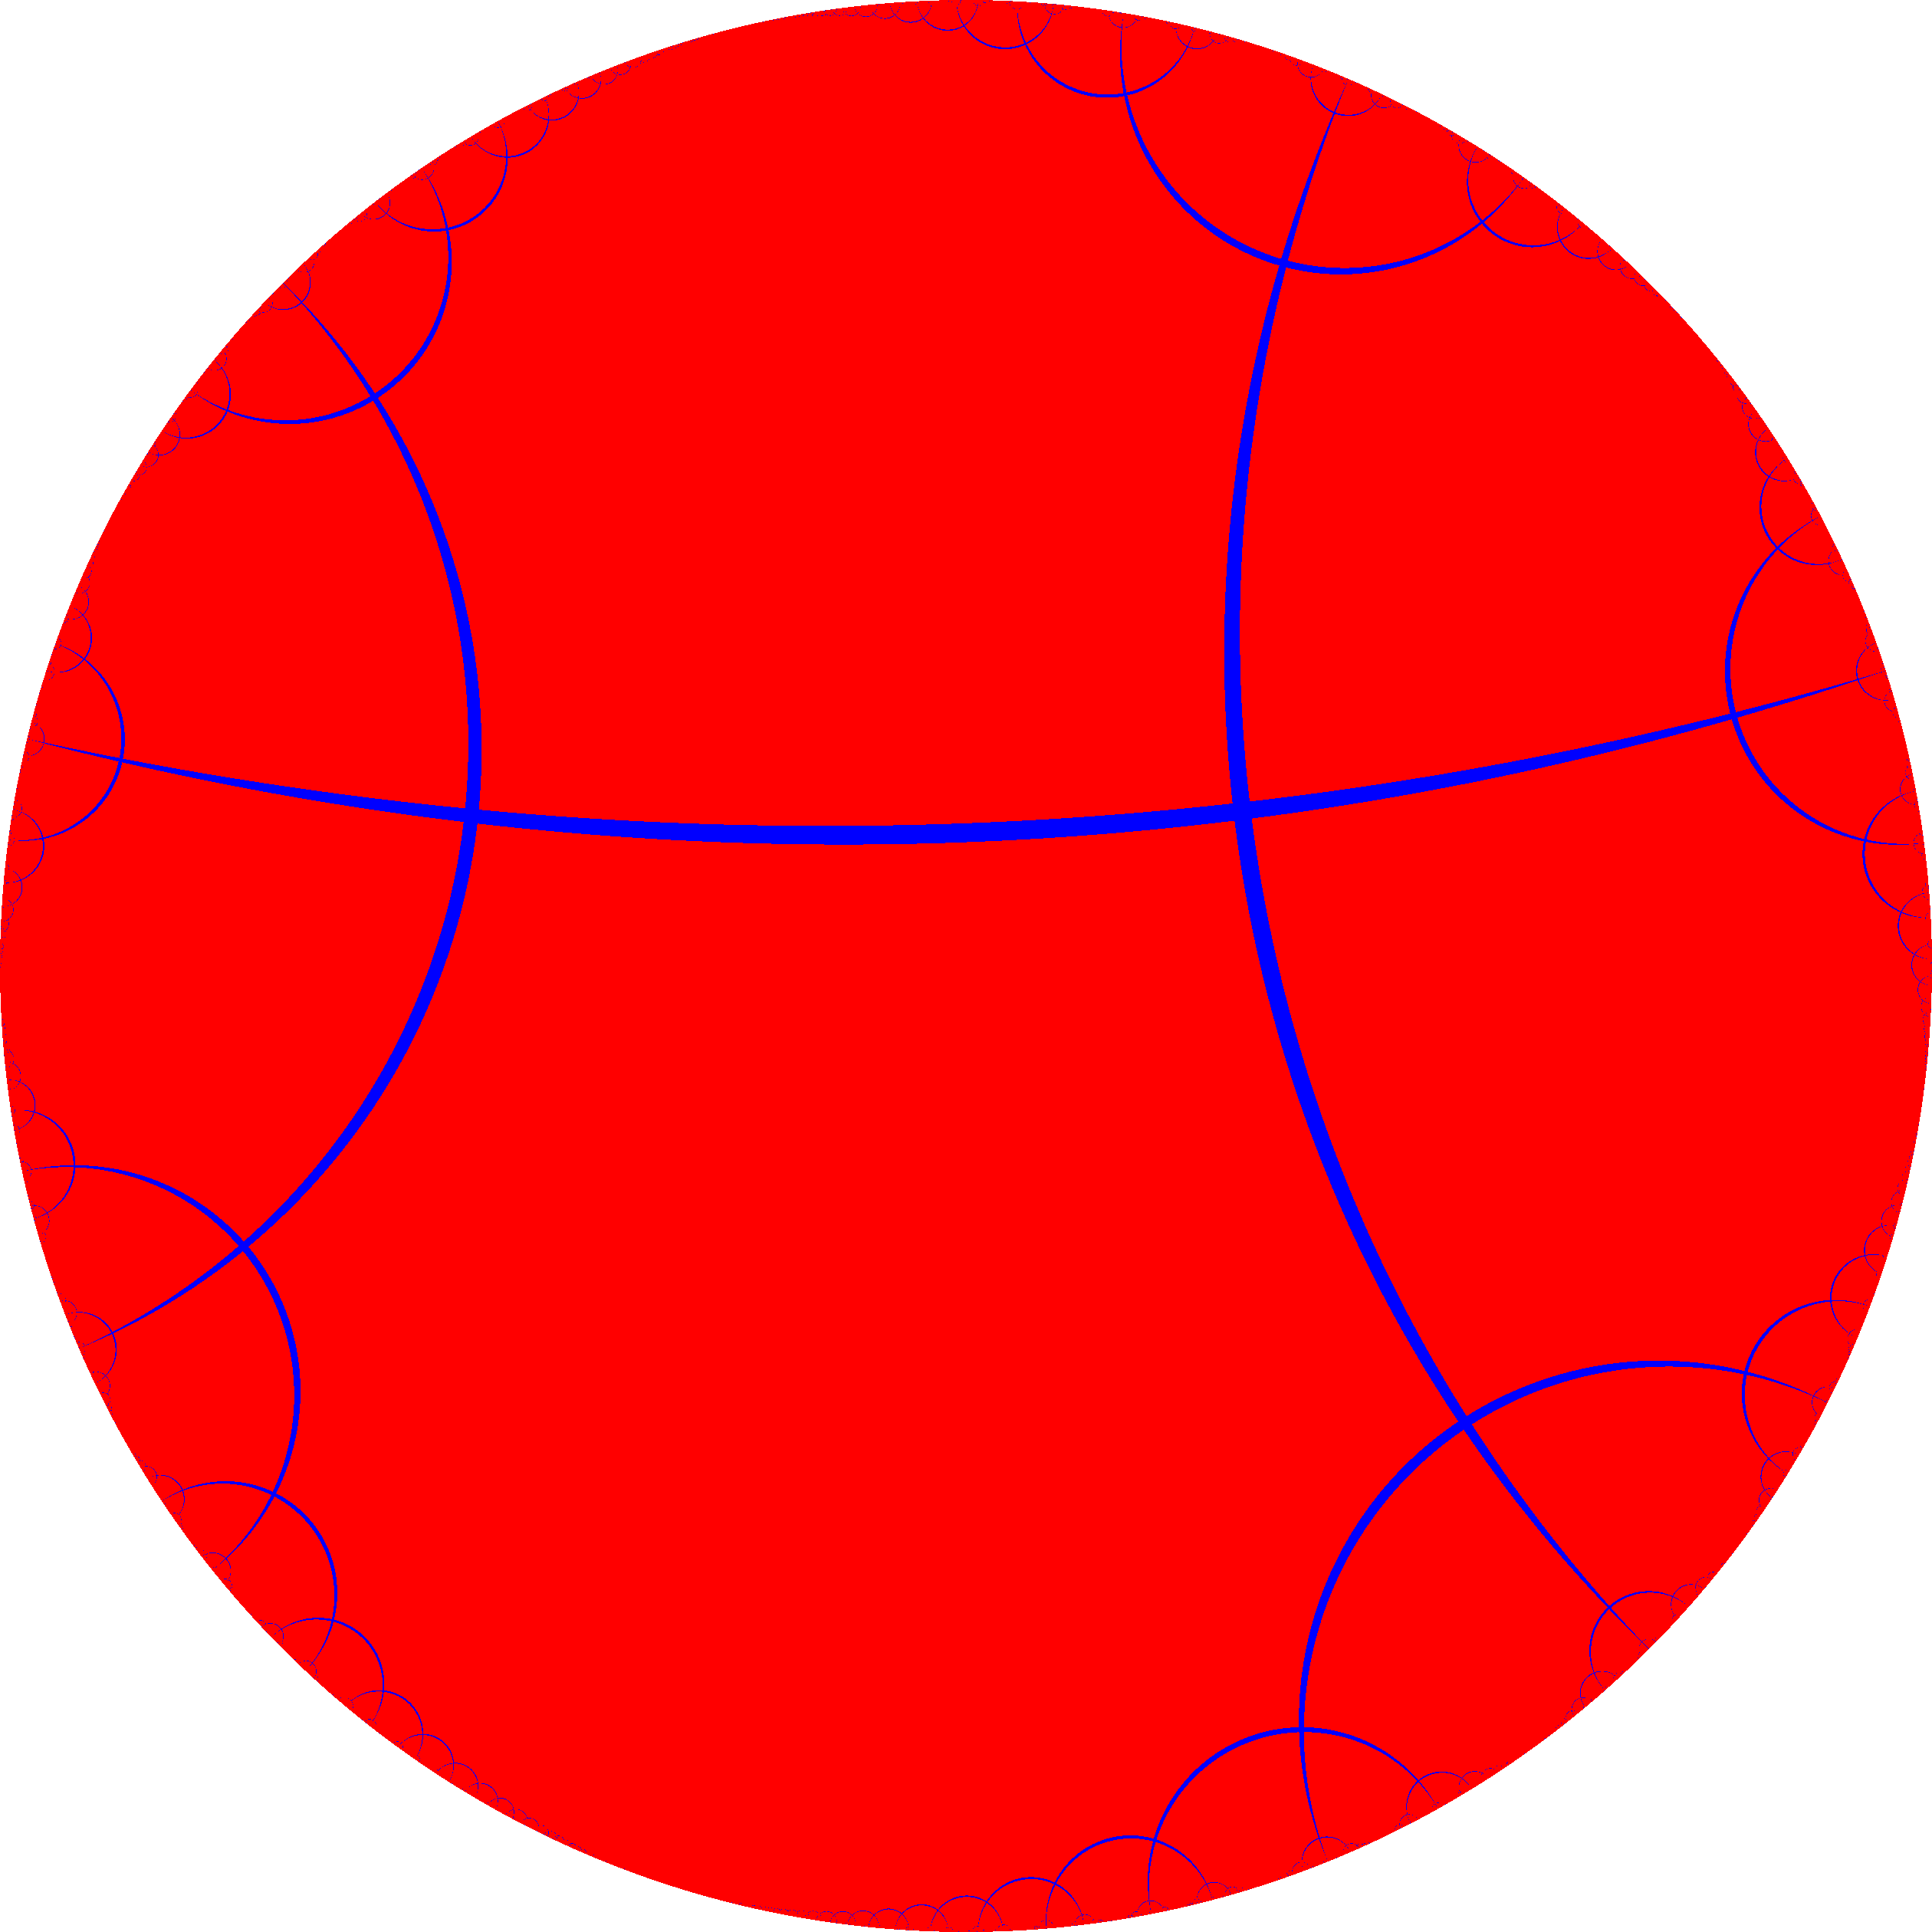
\includegraphics[width=4in]{images/H2_tiling_24i-1.png}
\caption{染色与定向}
\end{figure}

在上述染色的基础上,我们对边可以依照下述规则形成右手系排布:

\end{proof}

\section{代数的观点}

从数的角度讲,加减乘除四则运算的代数结构是域;但是从算术表达式的角度讲,四则运算对应到的代数结构是群。
由此引向算术表达式的路径群与典范形式的讨论。

最后,我们指出交换子的值和空间的弯曲程度相关。

\section{流方程}

假设在一个无穷小范围内存在算术表达式生成结构的一种几何,它会是什么样呢?本节我们探讨这个话题。

算术表达式空间中一点 $p$,$p$ 作为表达式有估值 $x$,假设在 $p$ 点存在加轴和乘轴构成的标架 $F_i$,
$p$ 有一个运动,在标架 $F_i$ 中表现为速度 $u$ 和角度 $\theta$ , 我们对 $p$ 的运动带来的估值 $x$ 的变化,
通过下述推导,可以建立方程

\begin{equation}
    x_{\delta} = (x_0 + \mu \epsilon \cos \theta)e^{\lambda \epsilon \sin \theta}
\end{equation}

或者

\begin{equation}
    x_{\delta} = x_0 e^{\lambda \epsilon \sin \theta} + \mu \epsilon \cos \theta
\end{equation}

两者都可以简化为

\begin{equation}
    x_{\delta} = x_0 + \epsilon (x_0 \lambda \sin \theta + \mu \cos \theta)
\end{equation}

于是

\begin{equation}
    \frac{1}{\delta} (x_{\delta} - x_0) = \frac{\epsilon}{\delta} (\mu \cos \theta + x_0 \lambda \sin \theta)
\end{equation}

当 $\delta$ 和 $\epsilon$ 同时趋于零时,我们就得到了 $dx / dt$,即有

\begin{equation}
    \frac{dx}{dt} = u (\mu \cos \theta + x \lambda \sin \theta)
\end{equation}

最后,我们指出流方程的推导是抽象的,我们在推导过程中并没有用上前面章节里具体的几何结构。

\section{管型构造}

\section{新的实例}

\section{可能的框架}

\newpage
\phantomsection
\addcontentsline{toc}{section}{参考文献}
\bibliographystyle{ieeetr}
\bibliography{biblio/article}

\end{document}


